% Presenting mathematics: a frame for watching past presentations, then the
% documentation questions that come up in the same week.
% Shared preamble for the write-on class slides.
%
% Every deck is designed to be projected and annotated live on a tablet:
% whatever takes time to draw is pre-drawn, and whatever the class produces is
% left blank. Compile a deck with `pdflatex main.tex` from its own directory,
% or run `uv run python build.py` from the repository root to build them all.
\documentclass[10pt]{article}

\usepackage[papersize={25.6cm,14.4cm}, margin=1.1cm, bottom=1.5cm,
            footskip=0.75cm]{geometry}
\usepackage[T1]{fontenc}
\usepackage[default]{sourcesanspro}
\usepackage{newtxsf}
\usepackage{tikz}
\usepackage{amsmath}
\usepackage{parskip}
\usepackage{fancyhdr}
\usetikzlibrary{arrows.meta, positioning, calc}

\setlength{\parindent}{0pt}

% Catppuccin Latte, the palette the course site uses in its light theme, so a
% deck on the projector looks like the pages the students read.
\definecolor{inkbg}{HTML}{EFF1F5}      % base
\definecolor{inksurface}{HTML}{E6E9EF} % mantle
\definecolor{inkfaint}{HTML}{CCD0DA}   % surface2, for rules and empty boxes
\definecolor{inktext}{HTML}{4C4F69}    % text
\definecolor{inkgrey}{HTML}{8C8FA1}    % overlay1, for anything secondary
\definecolor{inkblue}{HTML}{7287FD}    % lavender, the primary accent
\definecolor{inkteal}{HTML}{179299}    % teal
\definecolor{inkred}{HTML}{FE640B}     % peach, for whatever wants attention
\definecolor{inkmauve}{HTML}{8839EF}   % mauve

\pagecolor{inkbg}
\color{inktext}

% A box to write a short answer into. White against the tinted page, so it
% reads as somewhere to write rather than as part of the printed material.
\newcommand{\blank}[1][1.6]{%
  \tikz[baseline=(current bounding box.base)]{%
    \draw[inkfaint, line width=0.7pt, rounded corners=2pt, fill=white]
      (0,-0.18) rectangle (#1,0.62);}}

% A ruled area to work in. Faint dots keep handwriting level on a tablet.
\newcommand{\workspace}[2]{%
  \begin{tikzpicture}
    \draw[inkfaint, line width=0.7pt, rounded corners=3pt, fill=white]
      (0,0) rectangle (#1,#2);
    \foreach \gx in {0.5,1.0,...,#1}{%
      \foreach \gy in {0.5,1.0,...,#2}{%
        \fill[inkfaint] (\gx,\gy) circle (0.5pt);}}
  \end{tikzpicture}}

% A panel for material that is printed rather than written on.
\newcommand{\panel}[2]{%
  \begin{tikzpicture}
    \draw[inkfaint, line width=0.7pt, rounded corners=3pt, fill=inksurface]
      (0,0) rectangle (#1,#2);
  \end{tikzpicture}}

% A labelled card of printed material. #2 and #3 are widths in cm; the text
% column is the card less its padding, computed rather than guessed.
\newcommand{\cardbox}[4]{%
  \begin{tikzpicture}
    \node[draw=#1, line width=1pt, rounded corners=4pt, fill=white,
          minimum width=#2cm, minimum height=#3cm,
          text width=\dimexpr#2cm-0.9cm\relax,
          align=left, inner sep=0.45cm, text=inktext] {#4};
  \end{tikzpicture}}

% A card whose body is left blank for the class to fill in.
\newcommand{\cardblank}[4]{%
  \begin{tikzpicture}
    \node[draw=#1, line width=1pt, rounded corners=4pt, fill=white,
          minimum width=#2cm, minimum height=#3cm,
          text width=\dimexpr#2cm-0.9cm\relax,
          align=left, inner sep=0.45cm, text=inktext, anchor=north west]
      at (0,0) {#4};
  \end{tikzpicture}}

% Running header: the deck name on the left, the page's own step on the right.
% Each deck sets its name once with \deckname.
\newcommand{\deck}{}
\newcommand{\deckname}[1]{\renewcommand{\deck}{#1}}
\newcommand{\slidehead}[1]{%
  {\small\color{inkgrey}%
   \tikz[baseline=-0.5ex]{\fill[inkblue, rounded corners=1pt]
     (0,0) rectangle (0.22,0.22);}\;\deck
   \hfill \color{inkblue}\bfseries #1}\par
  {\color{inkblue}\rule{\linewidth}{1pt}}\par\vspace{0.35em}}

\pagestyle{fancy}
\fancyhf{}
\renewcommand{\headrulewidth}{0pt}
\fancyfoot[R]{\small\color{inkgrey}\thepage}

% Deck title pages, which carry no header and no page number.
\newcommand{\titleslide}[3]{%
  \thispagestyle{empty}%
  \begin{center}
    \vspace*{\fill}
    {\Huge\bfseries\color{inkblue} #1}\\[0.7em]
    {\LARGE\color{inkgrey} #2}\\[2.4em]
    #3
    \vspace*{\fill}
  \end{center}}

% One step of the plan on a title page.
\newcommand{\stepbox}[3]{%
  \node[draw=inkblue, line width=0.9pt, rounded corners=4pt, fill=white,
        minimum width=6cm, minimum height=1.7cm, align=center,
        text=inktext] (#1) at (#2,0) {#3};}

% Prompt to the room: a question the class answers, not something I read out.
\newcommand{\ask}[1]{%
  {\large\color{inkblue}\bfseries #1}\par\vspace{0.5em}}


\deckname{Presenting mathematics}

\begin{document}

\titleslide{Presenting mathematics}{Week 9. Three presentations, and what
you make of them.}{%
    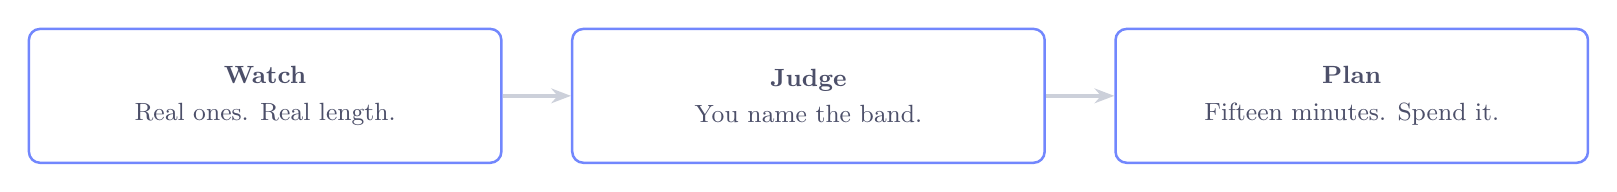
\begin{tikzpicture}[font=\small]
      \stepbox{s0}{0.0}{\textbf{Watch}\\[0.25em] Real ones. Real length.}
      \stepbox{s1}{6.9}{\textbf{Judge}\\[0.25em] You name the band.}
      \stepbox{s2}{13.8}{\textbf{Plan}\\[0.25em] Fifteen minutes. Spend it.}
      \draw[-{Stealth[length=2.5mm]}, inkfaint, line width=1.2pt] (s0) -- (s1);
      \draw[-{Stealth[length=2.5mm]}, inkfaint, line width=1.2pt] (s1) -- (s2);
    \end{tikzpicture}}

\newpage
\slidehead{A presentation is a performance}

\vspace{1.4cm}

\begin{center}
{\Huge\bfseries\color{inkblue} It is not your slides.}

\vspace{1.8cm}

{\LARGE If the audience could get everything from your visual aids\\
without you, you have written a document, not a talk.}
\end{center}

\newpage
\slidehead{Three more claims}

\vspace{1.2cm}

{\LARGE
\textbf{\color{inkblue}1.}\quad If you put up a visual aid, the audience
will look at it. So it had better be helping.

\vspace{1.2em}

\textbf{\color{inkteal}2.}\quad Less is more. A shorter presentation is
better than a longer one.

\vspace{1.2em}

\textbf{\color{inkred}3.}\quad Teaching and presenting are not the same
thing. You are not teaching us your library.}

\vspace{1.5cm}

\begin{center}
{\large\color{inkgrey} Your job is to spark interest, not to transfer
everything you know.}
\end{center}

\newpage
\slidehead{What to watch for}

\vspace{0.5cm}

\begin{center}
{\large
\begin{tabular}{@{}p{9.8cm}ccc@{}}
 & \textbf{\color{inkblue}One} & \textbf{\color{inkteal}Two}
   & \textbf{\color{inkred}Three}\\[0.5em]
Minutes before the library appeared & \blank[3.0] & \blank[3.0]
  & \blank[3.0]\\[2.1em]
Visual aids: working, or a transcript? & \blank[3.0] & \blank[3.0]
  & \blank[3.0]\\[2.1em]
What did you learn that the README would not tell you? & \blank[3.0]
  & \blank[3.0] & \blank[3.0]\\[2.1em]
Could you tell what each member had done? & \blank[3.0] & \blank[3.0]
  & \blank[3.0]\\[2.1em]
Which band? & \blank[3.0] & \blank[3.0] & \blank[3.0]\\
\end{tabular}}
\end{center}

\vspace{0.4cm}

{\small\color{inkgrey} These are real submissions for this exact piece of
coursework, shown with their groups' permission.}

\newpage
\slidehead{Communication is 30\% of the project mark}

\vspace{1.0cm}

{\LARGE
The paper and the presentation are marked \textbf{together}, on five
things:

\vspace{1.0em}

\textbf{\color{inkblue}Summary.}\quad
\textbf{\color{inkteal}Statement of need.}\quad
\textbf{\color{inkred}Quality of writing.}

\vspace{0.8em}

\textbf{\color{inkmauve}Functionality.}\quad
\textbf{\color{inkblue}Presentation and visual aids.}}

\vspace{1.5cm}

\begin{center}
{\large\color{inkgrey} A good paper and a rushed presentation cannot both
be true of the same group. The marker sees one mark.}
\end{center}

\newpage
\slidehead{Fifteen minutes. Spend it.}

\vspace{0.7cm}

{\LARGE
The problem, and why anyone cares \dotfill \blank[2.2]

\vspace{0.5em}

The mathematics \dotfill \blank[2.2]

\vspace{0.5em}

What the library does, and how it is built \dotfill \blank[2.2]

\vspace{0.5em}

The demonstration \dotfill \blank[2.2]

\vspace{0.5em}

What it does not do \dotfill \blank[2.2]}

\vspace{1.1cm}

{\small\color{inkgrey} Eleven minutes of mathematics and three of software
is the commonest way to lose this mark.}

\newpage
\slidehead{Scenes, not slides}

\vspace{1.0cm}

\begin{center}

\begin{tikzpicture}
  \foreach \x in {0, 5.75, 11.5, 17.25}{%
    \draw[inkfaint, line width=0.8pt, rounded corners=3pt, fill=white]
      (\x,0) rectangle (\x+5.2,2.9);
    \draw[inkfaint, line width=0.8pt, rounded corners=3pt, fill=white]
      (\x,-3.5) rectangle (\x+5.2,-0.6);}
\end{tikzpicture}
\end{center}

\vspace{1.0cm}

\ask{Storyboard it like a film. What are the eight scenes?}

\vspace{0.3cm}

{\small\color{inkgrey} A scene is not a slide. One scene may need three
slides, or none at all.}

\newpage
\slidehead{The demonstration is recorded}

\vspace{1.3cm}

\begin{center}
{\LARGE Nothing can fail live.\\[1.2em]
Which means a \textbf{failure that is still in the recording}\\
is worse than a live one.}
\end{center}

\vspace{1.6cm}

\begin{center}
{\large\color{inkgrey} Rehearse the demonstration once before you record
it. Then watch it back before you submit.}
\end{center}

\newpage
\slidehead{This week's reading}

\vspace{1.1cm}

\begin{center}
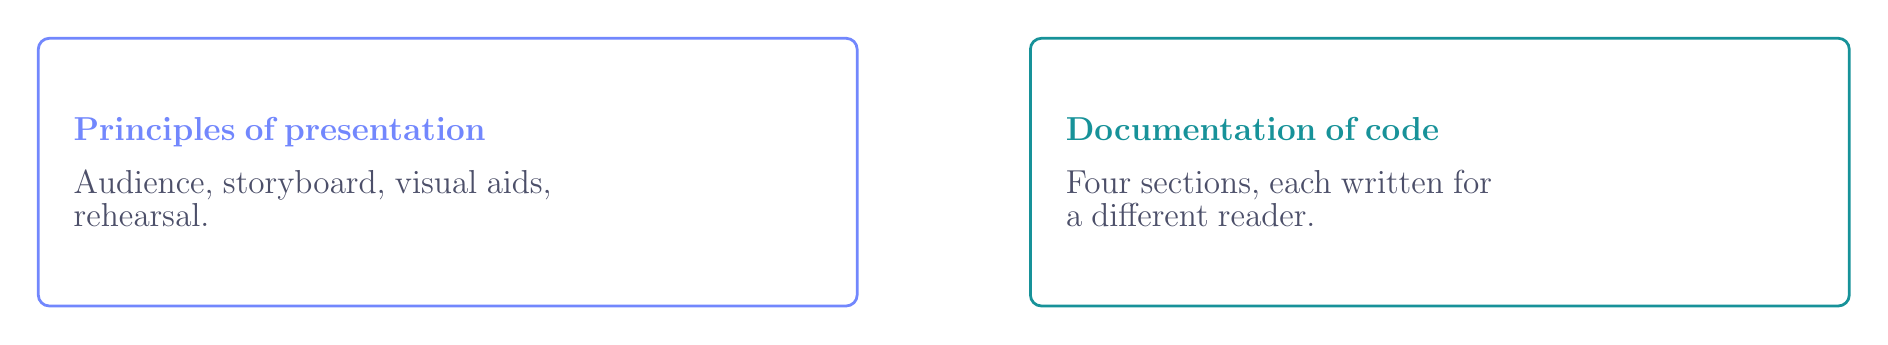
\begin{tikzpicture}
  \node at (0,0) {\cardbox{inkblue}{10.4}{3.4}{%
    {\large\bfseries\color{inkblue} Principles of presentation}\\[0.5em]
    {\large Audience, storyboard, visual aids,\\ rehearsal.}}};
  \node at (12.6,0) {\cardbox{inkteal}{10.4}{3.4}{%
    {\large\bfseries\color{inkteal} Documentation of code}\\[0.5em]
    {\large Four sections, each written for\\ a different reader.}}};
\end{tikzpicture}
\end{center}

\vspace{1.2cm}

\begin{center}
{\LARGE You read these \textbf{on your own}. The next three slides are the
parts that catch people.}
\end{center}

\newpage
\slidehead{Four sections. Which is which?}

\vspace{0.7cm}

\begin{center}
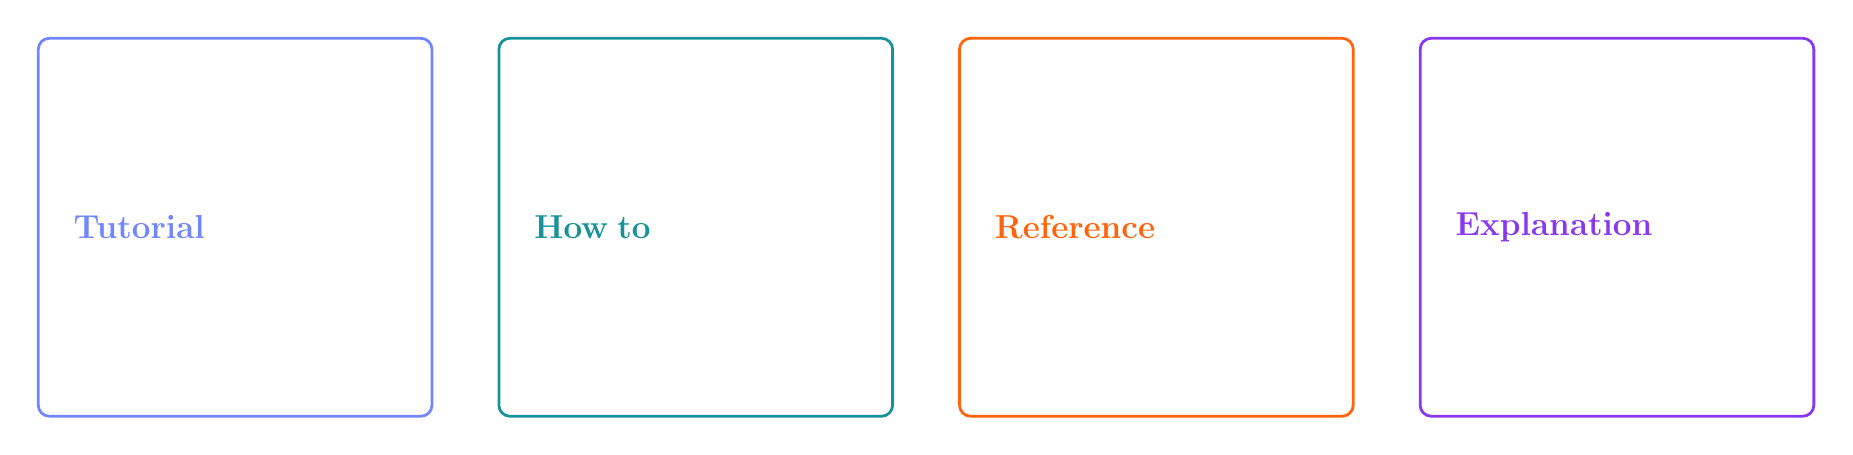
\begin{tikzpicture}
  \node at (0,0) {\cardblank{inkblue}{5.0}{4.8}{%
    {\large\bfseries\color{inkblue} Tutorial}}};
  \node at (5.85,0) {\cardblank{inkteal}{5.0}{4.8}{%
    {\large\bfseries\color{inkteal} How to}}};
  \node at (11.7,0) {\cardblank{inkred}{5.0}{4.8}{%
    {\large\bfseries\color{inkred} Reference}}};
  \node at (17.55,0) {\cardblank{inkmauve}{5.0}{4.8}{%
    {\large\bfseries\color{inkmauve} Explanation}}};
\end{tikzpicture}
\end{center}

\vspace{1.0cm}

\ask{A recipe. Your first time in a kitchen. Why a cooked onion tastes
sweet. Every ingredient in the cupboard, listed.}

\vspace{0.3cm}

{\small\color{inkgrey} To achieve a goal, to learn, to understand, to find
information. All four are in the Scope criterion.}

\newpage
\slidehead{README, or docstring?}

\vspace{0.9cm}

\begin{center}

\begin{tikzpicture}
  \node at (0,0) {\cardbox{inkblue}{10.4}{3.2}{%
    {\large\bfseries\color{inkblue} README.md}\\[0.5em]
    {\large Somebody deciding whether to\\ use your library, and learning
     how.}}};
  \node at (12.6,0) {\cardbox{inkteal}{10.4}{3.2}{%
    {\large\bfseries\color{inkteal} Docstrings}\\[0.5em]
    {\large Somebody reading one function,\\ inside the code.}}};
\end{tikzpicture}
\end{center}

\vspace{1.1cm}

\ask{You need both. Which of the two is a good variable name part of?}

\vspace{0.4cm}

{\small\color{inkgrey} Neither, and both. A name is documentation that
cannot go out of date.}

\newpage
\slidehead{How do you know it is enough?}

\vspace{1.3cm}

\begin{center}
{\LARGE\bfseries\color{inkblue} Give it to another group.}

\vspace{1.4cm}

{\LARGE The criterion is that your \texttt{README.md} would be usable by
somebody outside your group, with no help from you.}
\end{center}

\vspace{1.4cm}

\begin{center}
{\large\color{inkgrey} That is a test you can actually run, this week, in
ten minutes.}
\end{center}

\newpage
\slidehead{Before you leave}

\vspace{0.8cm}

\begin{center}
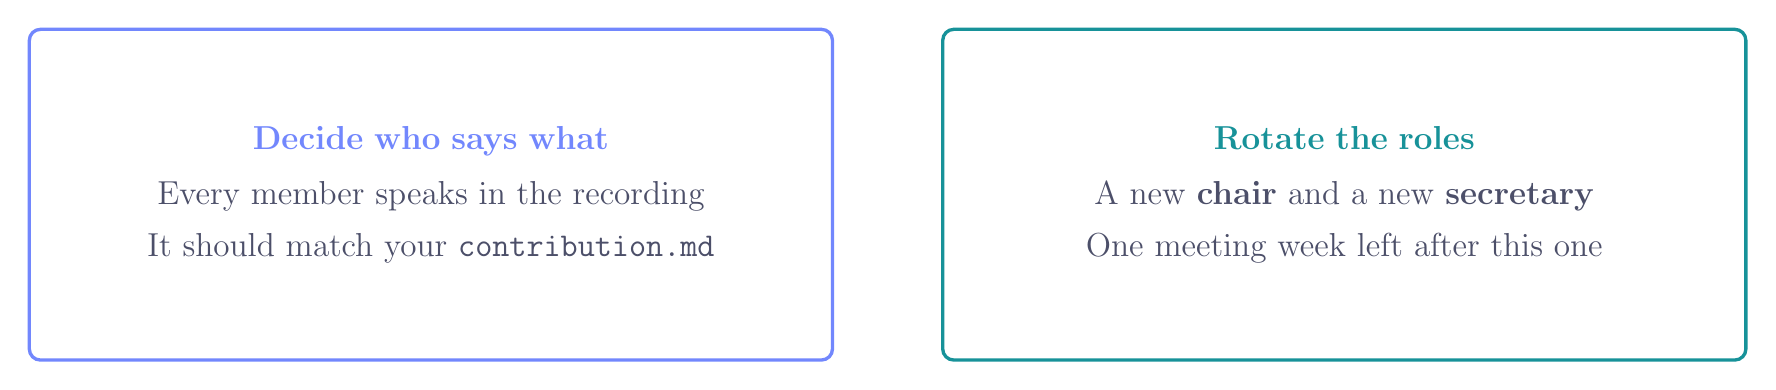
\begin{tikzpicture}
  \node[draw=inkblue, line width=1.2pt, rounded corners=4pt, fill=white,
        minimum width=10.2cm, minimum height=4.2cm, text width=9.2cm,
        align=center, inner sep=0.4cm, text=inktext, font=\large] at (0,0) {%
    \textbf{\color{inkblue} Decide who says what}\\[0.5em]
    Every member speaks in the recording\\[0.4em]
    It should match your
    \texttt{contribution.md}};
  \node[draw=inkteal, line width=1.2pt, rounded corners=4pt, fill=white,
        minimum width=10.2cm, minimum height=4.2cm, text width=9.2cm,
        align=center, inner sep=0.4cm, text=inktext, font=\large]
    at (11.6,0) {%
    \textbf{\color{inkteal} Rotate the roles}\\[0.5em]
    A new \textbf{chair} and a new \textbf{secretary}\\[0.4em]
    One meeting week left after this one};
\end{tikzpicture}
\end{center}

\vspace{0.9cm}

\begin{center}

\begin{tikzpicture}
  \node[draw=inkred, line width=1.4pt, rounded corners=4pt, fill=white,
        minimum width=21.8cm, minimum height=2.2cm, text width=20.6cm,
        align=center, inner sep=0.35cm, text=inktext, font=\large] {%
    \textbf{\color{inkred} Meet this week. Bring the Week 9 minutes to the
    next session.}\quad The fourth of the five that \(I\) is counted from.};
\end{tikzpicture}
\end{center}

\end{document}
